\documentclass{article}\usepackage[]{graphicx}\usepackage[]{color}
% maxwidth is the original width if it is less than linewidth
% otherwise use linewidth (to make sure the graphics do not exceed the margin)
\makeatletter
\def\maxwidth{ %
  \ifdim\Gin@nat@width>\linewidth
    \linewidth
  \else
    \Gin@nat@width
  \fi
}
\makeatother

\definecolor{fgcolor}{rgb}{0.345, 0.345, 0.345}
\newcommand{\hlnum}[1]{\textcolor[rgb]{0.686,0.059,0.569}{#1}}%
\newcommand{\hlstr}[1]{\textcolor[rgb]{0.192,0.494,0.8}{#1}}%
\newcommand{\hlcom}[1]{\textcolor[rgb]{0.678,0.584,0.686}{\textit{#1}}}%
\newcommand{\hlopt}[1]{\textcolor[rgb]{0,0,0}{#1}}%
\newcommand{\hlstd}[1]{\textcolor[rgb]{0.345,0.345,0.345}{#1}}%
\newcommand{\hlkwa}[1]{\textcolor[rgb]{0.161,0.373,0.58}{\textbf{#1}}}%
\newcommand{\hlkwb}[1]{\textcolor[rgb]{0.69,0.353,0.396}{#1}}%
\newcommand{\hlkwc}[1]{\textcolor[rgb]{0.333,0.667,0.333}{#1}}%
\newcommand{\hlkwd}[1]{\textcolor[rgb]{0.737,0.353,0.396}{\textbf{#1}}}%
\let\hlipl\hlkwb

\usepackage{framed}
\makeatletter
\newenvironment{kframe}{%
 \def\at@end@of@kframe{}%
 \ifinner\ifhmode%
  \def\at@end@of@kframe{\end{minipage}}%
  \begin{minipage}{\columnwidth}%
 \fi\fi%
 \def\FrameCommand##1{\hskip\@totalleftmargin \hskip-\fboxsep
 \colorbox{shadecolor}{##1}\hskip-\fboxsep
     % There is no \\@totalrightmargin, so:
     \hskip-\linewidth \hskip-\@totalleftmargin \hskip\columnwidth}%
 \MakeFramed {\advance\hsize-\width
   \@totalleftmargin\z@ \linewidth\hsize
   \@setminipage}}%
 {\par\unskip\endMakeFramed%
 \at@end@of@kframe}
\makeatother

\definecolor{shadecolor}{rgb}{.97, .97, .97}
\definecolor{messagecolor}{rgb}{0, 0, 0}
\definecolor{warningcolor}{rgb}{1, 0, 1}
\definecolor{errorcolor}{rgb}{1, 0, 0}
\newenvironment{knitrout}{}{} % an empty environment to be redefined in TeX

\usepackage{alltt}
\title{Oppgaver R-seminar 4
  \linebreak STV1020 -- VÅREN 2021}
\author{Louisa Boulaziz}
\date{\today}
\IfFileExists{upquote.sty}{\usepackage{upquote}}{}
\begin{document}
\maketitle

\section{OPPGAVER}
\begin{enumerate}
\item Last inn datasettet "VALGDATA.Rdata"
\item Hva er navnene på variablene i datasettet? 
\item Hvor mang missing er det totalt i datasettet?
\item Hvor mange missing er det på hver enkelt variabel?
\item Lag et subset av dataene hvor du fjerner NA på variabelen valg.
\item Hvor mange kvinner og hvor mange menn er det i datasettet?
\item Gjør variabelen alder og kjønn til numerisk.
\item Finn gjennomsnittsalderen. 
\item Finn gjennomsnittsalderen til henholdsvis menn og kvinner. Regn ut forskjellen.
\item Få oversikt over variablen valg. Lag en oversikt som viser den univariate fordelingen -- hvor mange har stemt på hvert av partiene?
\item Finn korrelasjonen mellom alder og rik. 
\item Lag et spredningsdiagram mellom alder og rik med støttelinje. Endre navnene på x-aksen, y-aksen, og gi diagrammet en tittel. Tolk form, retning og styrke.


\end{enumerate}

\hfill \break \textbf{Variabler}
\begin{enumerate}
\item rik -- hvor viktig er det å være rik, ha penger og dyre ting? (1-6), 1 = helt enig, 6 = helt uenig 
\item alder -- i antall år
\item kjonn -- dikotom, 1 = mann, 2 = kvinne
\item tillit -- tillit til politikere, (1-10), 1 = ikke noe tillit, 10 = full tillit
\item valg -- hvilket parti stemte du ved forrige stortingsvalg
\item redusere -- Er du enig i at regjeringen skal omfordele goder. (1-5), 1 = veldig enig, 5 = helt uenig.
\end{enumerate}


\newpage 
\section{FASIT}
\begin{enumerate}
\item Last inn datasettet "VALGDATA.Rdata" og last inn pakken "tidyverse"
\begin{knitrout}
\definecolor{shadecolor}{rgb}{0.969, 0.969, 0.969}\color{fgcolor}\begin{kframe}
\begin{alltt}
\hlkwd{load}\hlstd{(}\hlstr{"VALGDATA.Rdata"}\hlstd{)}

\hlcom{# Bytter navn}

\hlstd{data} \hlkwb{<-} \hlstd{nyedata}

\hlcom{# Fjerner den andre }

\hlkwd{rm}\hlstd{(nyedata)}

\hlcom{# Pakke }

\hlkwd{library}\hlstd{(tidyverse)}
\end{alltt}


{\ttfamily\noindent\itshape\color{messagecolor}{\#\# -- Attaching packages --------------------------------------- tidyverse 1.3.0 --}}

{\ttfamily\noindent\itshape\color{messagecolor}{\#\# v ggplot2 3.3.3\ \ \ \  v purrr\ \  0.3.4\\\#\# v tibble\ \ 3.0.6\ \ \ \  v dplyr\ \  1.0.3\\\#\# v tidyr\ \  1.1.2\ \ \ \  v stringr 1.4.0\\\#\# v readr\ \  1.4.0\ \ \ \  v forcats 0.5.0}}

{\ttfamily\noindent\itshape\color{messagecolor}{\#\# -- Conflicts ------------------------------------------ tidyverse\_conflicts() --\\\#\# x dplyr::filter() masks stats::filter()\\\#\# x dplyr::lag()\ \ \ \ masks stats::lag()}}\end{kframe}
\end{knitrout}

\item Hva er navnene på variablene i datasettet? 

\begin{knitrout}
\definecolor{shadecolor}{rgb}{0.969, 0.969, 0.969}\color{fgcolor}\begin{kframe}
\begin{alltt}
\hlkwd{show}\hlstd{(}\hlkwd{variable.names}\hlstd{(data))}
\end{alltt}
\begin{verbatim}
## [1] "rik"      "alder"    "kjonn"    "tillit"   "valg"     "redusere"
\end{verbatim}
\end{kframe}
\end{knitrout}
\item Hvor mang missing er det totalt i datasettet?

\begin{knitrout}
\definecolor{shadecolor}{rgb}{0.969, 0.969, 0.969}\color{fgcolor}\begin{kframe}
\begin{alltt}
\hlkwd{sum}\hlstd{(}\hlkwd{is.na}\hlstd{(data))}
\end{alltt}
\begin{verbatim}
## [1] 377
\end{verbatim}
\end{kframe}
\end{knitrout}
\item Hvor mange missing er det på hver enkelt variabel?

\begin{knitrout}
\definecolor{shadecolor}{rgb}{0.969, 0.969, 0.969}\color{fgcolor}\begin{kframe}
\begin{alltt}
\hlkwd{summary}\hlstd{(data)}
\end{alltt}
\begin{verbatim}
##       rik            alder          kjonn           tillit     
##  Min.   :1.000   Min.   :15.0   Min.   :1.000   Min.   : 0.00  
##  1st Qu.:4.000   1st Qu.:32.0   1st Qu.:1.000   1st Qu.: 4.00  
##  Median :5.000   Median :47.5   Median :1.000   Median : 5.00  
##  Mean   :4.558   Mean   :47.1   Mean   :1.447   Mean   : 5.28  
##  3rd Qu.:5.000   3rd Qu.:61.0   3rd Qu.:2.000   3rd Qu.: 7.00  
##  Max.   :6.000   Max.   :90.0   Max.   :2.000   Max.   :10.00  
##  NA's   :7       NA's   :32                     NA's   :8      
##      valg              redusere    
##  Length:1406        Min.   :1.000  
##  Class :character   1st Qu.:2.000  
##  Mode  :character   Median :2.000  
##                     Mean   :2.194  
##                     3rd Qu.:3.000  
##                     Max.   :5.000  
##                     NA's   :7
\end{verbatim}
\begin{alltt}
\hlcom{# Eventuelt en for en }

\hlkwd{sum}\hlstd{(}\hlkwd{is.na}\hlstd{(data}\hlopt{$}\hlstd{redusere))}
\end{alltt}
\begin{verbatim}
## [1] 7
\end{verbatim}
\begin{alltt}
\hlkwd{sum}\hlstd{(}\hlkwd{is.na}\hlstd{(data}\hlopt{$}\hlstd{valg))}
\end{alltt}
\begin{verbatim}
## [1] 323
\end{verbatim}
\end{kframe}
\end{knitrout}
Variable som har målenivå "character" viser ikke NA i funksjonen "summary(data)"

\item Lag et subset av dataene hvor du fjerner NA på variabelen valg

\begin{knitrout}
\definecolor{shadecolor}{rgb}{0.969, 0.969, 0.969}\color{fgcolor}\begin{kframe}
\begin{alltt}
\hlstd{df} \hlkwb{<-} \hlstd{data} \hlopt
  \hlkwd{drop_na}\hlstd{(valg)}

\hlkwd{sum}\hlstd{(}\hlkwd{is.na}\hlstd{(data}\hlopt{$}\hlstd{valg))} \hlcom{# sjekker at det blir riktig }
\end{alltt}
\begin{verbatim}
## [1] 323
\end{verbatim}
\begin{alltt}
\hlnum{1406}\hlopt{-}\hlnum{323} \hlcom{# regner ut }
\end{alltt}
\begin{verbatim}
## [1] 1083
\end{verbatim}
\end{kframe}
\end{knitrout}
\item Hvor mange kvinner og hvor mange menn er det i datasettet?

\begin{knitrout}
\definecolor{shadecolor}{rgb}{0.969, 0.969, 0.969}\color{fgcolor}\begin{kframe}
\begin{alltt}
\hlkwd{table}\hlstd{(data}\hlopt{$}\hlstd{kjonn)}
\end{alltt}
\begin{verbatim}
## 
##   1   2 
## 777 629
\end{verbatim}
\end{kframe}
\end{knitrout}

\item Gjør variabelen alder og kjønn til numerisk.

\begin{knitrout}
\definecolor{shadecolor}{rgb}{0.969, 0.969, 0.969}\color{fgcolor}\begin{kframe}
\begin{alltt}
\hlkwd{class}\hlstd{(df}\hlopt{$}\hlstd{alder)}
\end{alltt}
\begin{verbatim}
## [1] "haven_labelled"
\end{verbatim}
\begin{alltt}
\hlstd{df}\hlopt{$}\hlstd{alder} \hlkwb{<-} \hlkwd{as.numeric}\hlstd{(df}\hlopt{$}\hlstd{alder)}

\hlkwd{class}\hlstd{(df}\hlopt{$}\hlstd{kjonn)}
\end{alltt}
\begin{verbatim}
## [1] "haven_labelled"
\end{verbatim}
\begin{alltt}
\hlstd{df}\hlopt{$}\hlstd{kjonn} \hlkwb{<-} \hlkwd{as.numeric}\hlstd{(df}\hlopt{$}\hlstd{kjonn)}
\end{alltt}
\end{kframe}
\end{knitrout}
\item Finn gjennomsnittsalderen. 

\begin{knitrout}
\definecolor{shadecolor}{rgb}{0.969, 0.969, 0.969}\color{fgcolor}\begin{kframe}
\begin{alltt}
\hlkwd{mean}\hlstd{(df}\hlopt{$}\hlstd{alder,} \hlkwc{na.rm} \hlstd{=} \hlnum{TRUE}\hlstd{)}
\end{alltt}
\begin{verbatim}
## [1] 50.45677
\end{verbatim}
\end{kframe}
\end{knitrout}
\item Finn gjennomsnittsalderen til henholdsvis menn og kvinner. Regn ut forskjellen.

\begin{knitrout}
\definecolor{shadecolor}{rgb}{0.969, 0.969, 0.969}\color{fgcolor}\begin{kframe}
\begin{alltt}
\hlstd{menn} \hlkwb{<-} \hlkwd{mean}\hlstd{(df}\hlopt{$}\hlstd{alder[df}\hlopt{$}\hlstd{kjonn} \hlopt{==} \hlnum{1}\hlstd{],} \hlkwc{na.rm} \hlstd{= T)}
\hlstd{menn}
\end{alltt}
\begin{verbatim}
## [1] 51.2381
\end{verbatim}
\begin{alltt}
\hlstd{kvinner} \hlkwb{<-} \hlkwd{mean}\hlstd{(df}\hlopt{$}\hlstd{alder[df}\hlopt{$}\hlstd{kjonn} \hlopt{==} \hlnum{2}\hlstd{],} \hlkwc{na.rm} \hlstd{= T)}
\hlstd{kvinner}
\end{alltt}
\begin{verbatim}
## [1] 49.4916
\end{verbatim}
\begin{alltt}
\hlstd{diff}\hlkwb{<-} \hlkwd{mean}\hlstd{(df}\hlopt{$}\hlstd{alder[df}\hlopt{$}\hlstd{kjonn} \hlopt{==} \hlnum{1}\hlstd{],} \hlkwc{na.rm} \hlstd{= T)} \hlopt{-} \hlkwd{mean}\hlstd{(df}\hlopt{$}\hlstd{alder[df}\hlopt{$}\hlstd{kjonn} \hlopt{==} \hlnum{2}\hlstd{],} \hlkwc{na.rm} \hlstd{= T)}

\hlstd{diff}
\end{alltt}
\begin{verbatim}
## [1] 1.746499
\end{verbatim}
\end{kframe}
\end{knitrout}


\item Få oversikt over variablen valg. Lag en oversikt som viser den univariate fordelingen -- hvor mange har stemt på hvert av partiene?

\begin{knitrout}
\definecolor{shadecolor}{rgb}{0.969, 0.969, 0.969}\color{fgcolor}\begin{kframe}
\begin{alltt}
\hlkwd{table}\hlstd{(df}\hlopt{$}\hlstd{valg)}
\end{alltt}
\begin{verbatim}
## 
##   Ap  Frp    H  Krf  MDG Rodt   Sp   SV    V 
##  302  102  304   46   45   30   89   98   67
\end{verbatim}
\begin{alltt}
\hlkwd{ggplot}\hlstd{(df,} \hlkwd{aes}\hlstd{(valg))} \hlopt{+}
  \hlkwd{geom_bar}\hlstd{()}
\end{alltt}
\end{kframe}
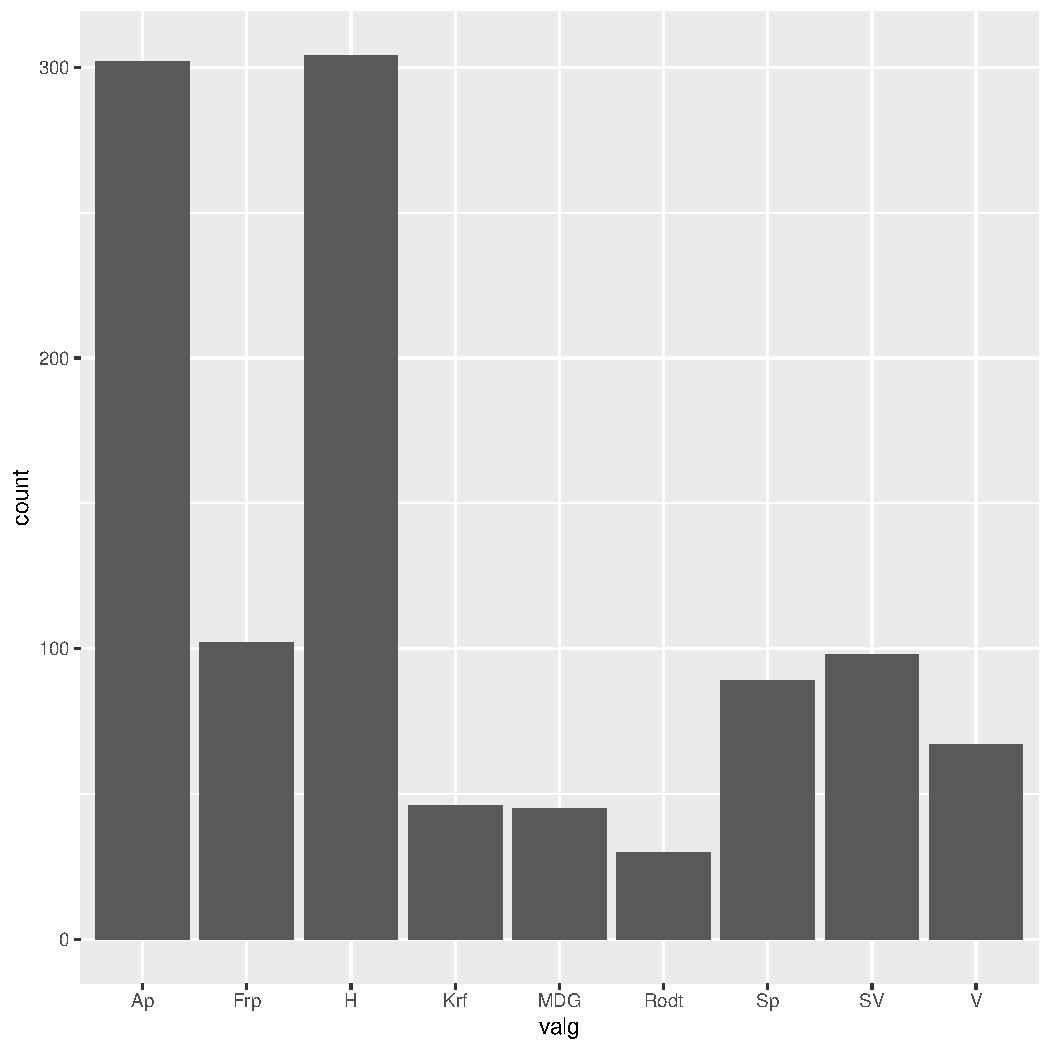
\includegraphics[width=\maxwidth]{figure/10-1} 

\end{knitrout}

\item Finn korrelasjonen mellom alder og rik. 
\begin{knitrout}
\definecolor{shadecolor}{rgb}{0.969, 0.969, 0.969}\color{fgcolor}\begin{kframe}
\begin{alltt}
\hlkwd{cor}\hlstd{(}\hlkwc{x}\hlstd{= df}\hlopt{$}\hlstd{rik,}
    \hlkwc{y}\hlstd{= df}\hlopt{$}\hlstd{alder,}
    \hlkwc{use} \hlstd{=} \hlstr{"pairwise.complete.obs"}\hlstd{)}
\end{alltt}
\begin{verbatim}
## [1] 0.3177088
\end{verbatim}
\end{kframe}
\end{knitrout}

\item Lag et spredningsdiagram mellom alder og rik med støttelinje. Endre på navnene på x-aksen, y-aksen, og gi diagrammet en tittel. Tolk form, retning og styrke.

\begin{knitrout}
\definecolor{shadecolor}{rgb}{0.969, 0.969, 0.969}\color{fgcolor}\begin{kframe}
\begin{alltt}
\hlcom{# Lager plot med støttelinje}
\hlkwd{scatter.smooth}\hlstd{(df}\hlopt{$}\hlstd{rik} \hlopt{~} \hlstd{df}\hlopt{$}\hlstd{alder,}
               \hlkwc{main} \hlstd{=} \hlstr{"Spredningsdiagram for alder og 
               viktigheten av å være rik"}\hlstd{,}
               \hlkwc{xlab} \hlstd{=} \hlstr{"Alder"}\hlstd{,}
               \hlkwc{ylab} \hlstd{=} \hlstr{"Viktigheten av å være rik"}\hlstd{)}
\end{alltt}
\end{kframe}
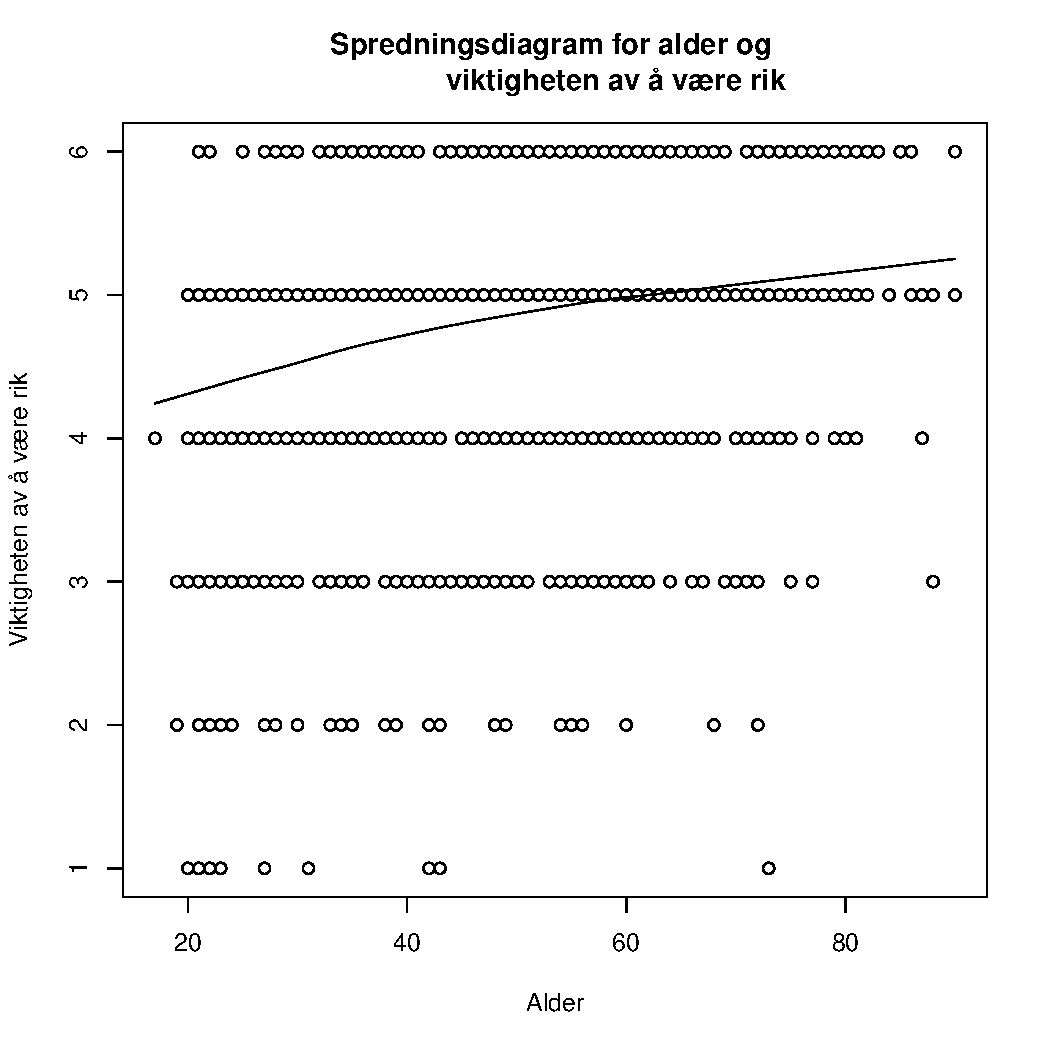
\includegraphics[width=\maxwidth]{figure/12-1} 
\begin{kframe}\begin{alltt}
\hlcom{# Ingen svært tydelig gruppering langs en rett linje}
\hlcom{# Positiv sammenheng. (0.32)}
\hlcom{# Jo eldre man blir, jo mindre viktig blir det å a være rik, }
\hlcom{# ha penger og dyre ting. }
\hlcom{# Men svak sammenheng. 0.32. }
\end{alltt}
\end{kframe}
\end{knitrout}

\end{enumerate}

\end{document}
